\chapter{Syslog}\label{syslog}

\section{Syslog Overview}\label{syslog-overview}

\begin{itemize}
\tightlist
\item
  SYSLOG is an INDUSTRY-STANDARD PROTOCOL for message logging
\item
  On NETWORK DEVICES, SYSLOG can be used to LOG EVENTS

  \begin{itemize}
  \tightlist
  \item
    Changes in INTERFACE status (UP / DOWN)
  \item
    Changes in OSFP NEIGHBOUR STATUS (UP / DOWN)
  \item
    System Restarts
  \item
    etc\ldots{}
  \end{itemize}
\item
  The messages can be displayed in the CLI, saved in the DEVICE'S RAM or
  sent to an external SYSLOG SERVER
\end{itemize}

\begin{figure}
\centering
\pandocbounded{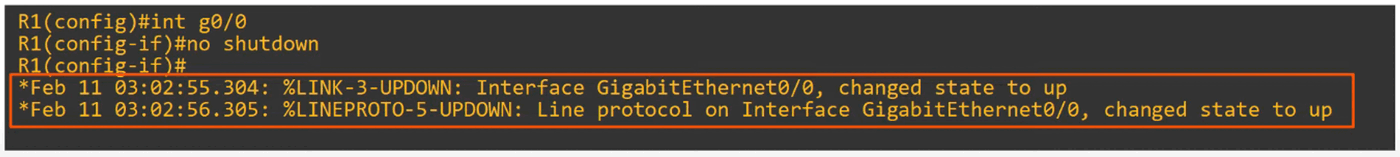
\includegraphics[keepaspectratio,alt={image}]{images/42-syslog/img-001.png}}
\end{figure}

\begin{itemize}
\tightlist
\item
  Logs are essential when troubleshooting issues, examining the cause of
  incidents, etc.
\item
  SYSLOG and SNMP are both used for MONITORING and TROUBLESHOOTING of
  DEVICES. They are complementary, but their functionalities are
  different
\end{itemize}

\section{Syslog Message Format}\label{syslog-message-format}

\passthrough{\lstinline!seq: time stamp: \%facility-severity-MNEMONIC:description!}

\begin{tipbox}

These TWO FIELDS may or may not be displayed, depending on the DEVICE'S
configuration

\end{tipbox}

\passthrough{\lstinline!seq!} = A SEQUENCE NUMBER indicating the order /
sequence of messages

\passthrough{\lstinline!time stamp!} = A TIMESTAMP indicating the time
the message was generated

\passthrough{\lstinline!facility!} = A VALUE that indicates which
process on the DEVICE generated the message

\passthrough{\lstinline!severity!} = A NUMBER that indicates the
severity of a logged event.

Official RFC for SYSLOG severity levels

\begin{tipbox}

LEVELS and KEYWORDS need to be MEMORIZED for the CCNA

\end{tipbox}

\begin{figure}
\centering
\pandocbounded{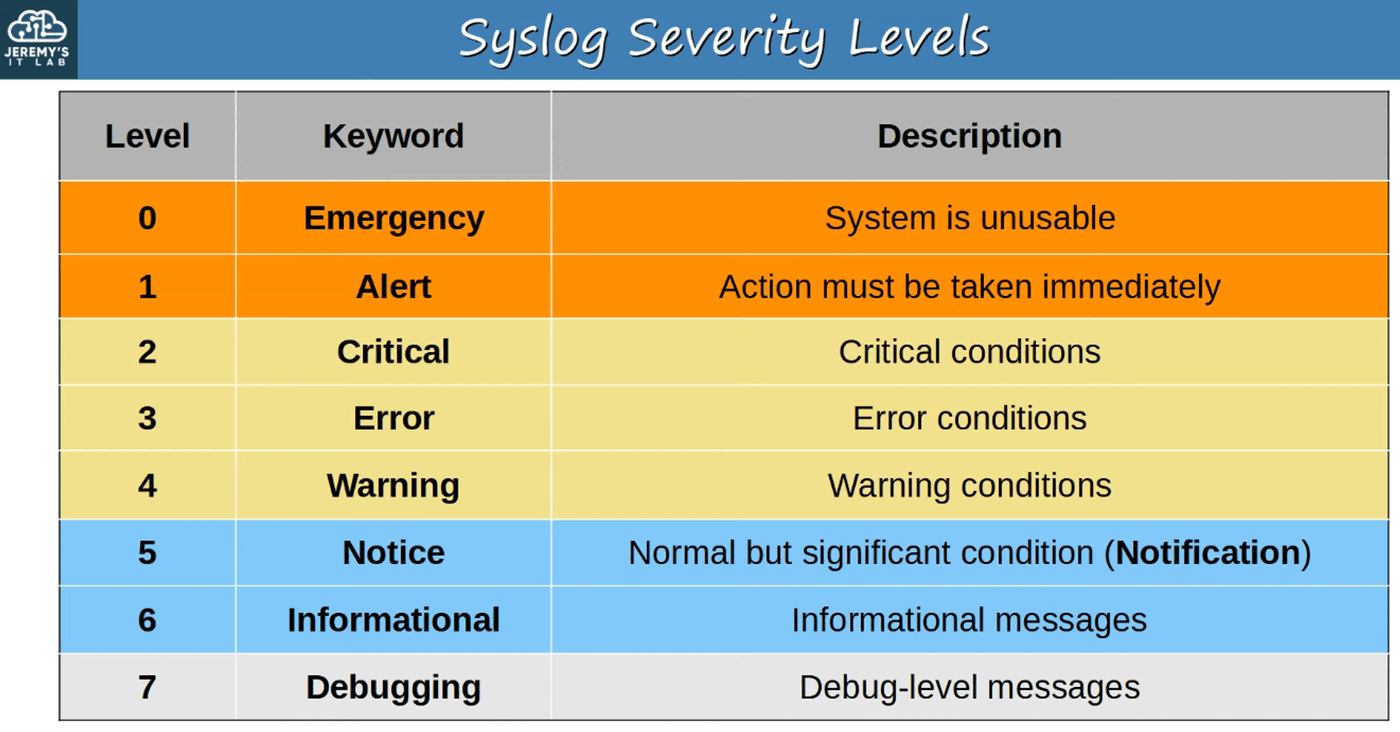
\includegraphics[keepaspectratio,alt={image}]{images/42-syslog/img-002.png}}
\end{figure}

\begin{tipbox}

MEMORIZATION MNEMONIC : (E)very (A)wesome (C)isco (E)ngineer (W)ill
(N)eed (I)ce cream (D)aily

\end{tipbox}

\passthrough{\lstinline!MNEMONIC!} = A SHORT CODE for the message,
indicating what happened

\passthrough{\lstinline!description!} = Detailed information about the
EVENT being reported

\begin{figure}
\centering
\pandocbounded{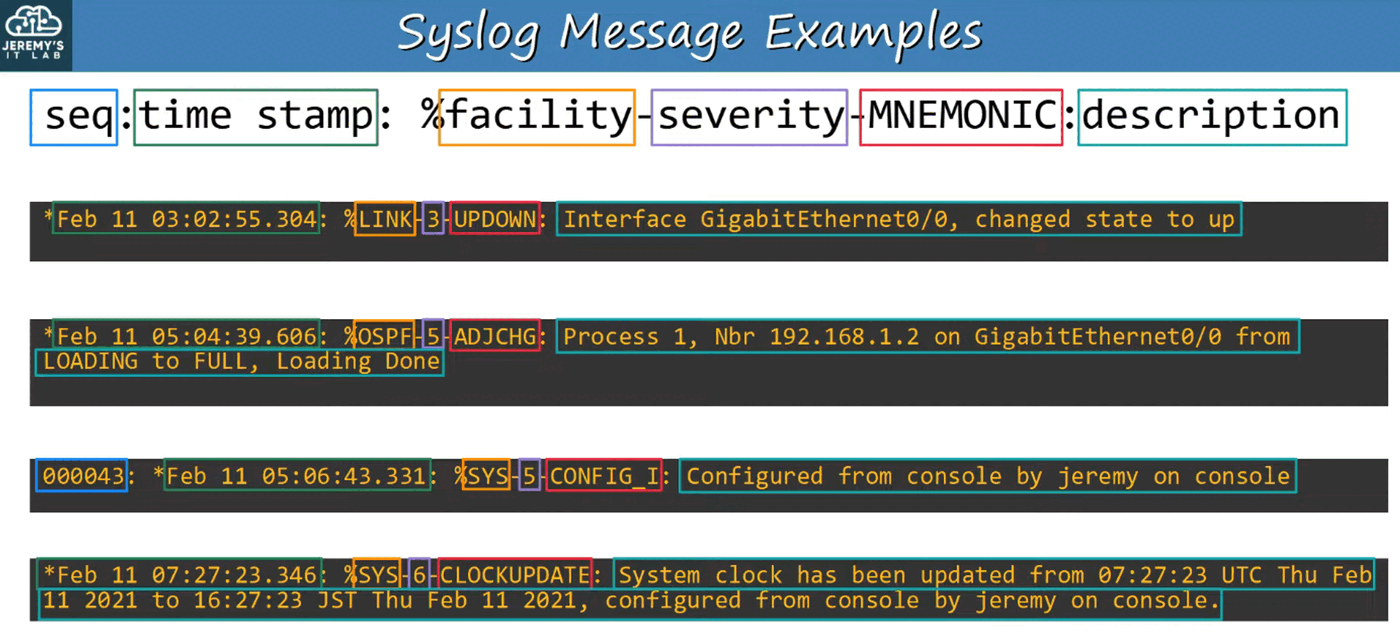
\includegraphics[keepaspectratio,alt={image}]{images/42-syslog/img-003.png}}
\end{figure}

\section{Syslog Logging Locations}\label{syslog-logging-locations}

\begin{itemize}
\tightlist
\item
  \textbf{CONSOLE LINE}

  \begin{itemize}
  \tightlist
  \item
    SYSLOG messages will be displayed in the CLI when connected to the
    DEVICE via the CONSOLE port. By DEFAULT, all messages (Level 0-7)
    are displayed
  \end{itemize}
\item
  \textbf{BUFFER}

  \begin{itemize}
  \tightlist
  \item
    Syslog messages will be saved to RAM. By default, ALL messages
    (Level 0-7) are displayed
  \end{itemize}
\item
  \textbf{VTY LINES}

  \begin{itemize}
  \tightlist
  \item
    SYSLOG messages will be displayed in the CLI when connected to the
    DEVICE via Telnet/SSH (coming in a later video). Disabled by
    default.
  \end{itemize}
\item
  \textbf{EXTERNAL SERVER}

  \begin{itemize}
  \tightlist
  \item
    You can configure the DEVICE to send SYSLOG messages to an external
    server
  \end{itemize}
\end{itemize}

** SYSLOG SERVERS will listen for messages on UDP PORT 514 **

\section{Syslog Configuration}\label{syslog-configuration}

\begin{figure}
\centering
\pandocbounded{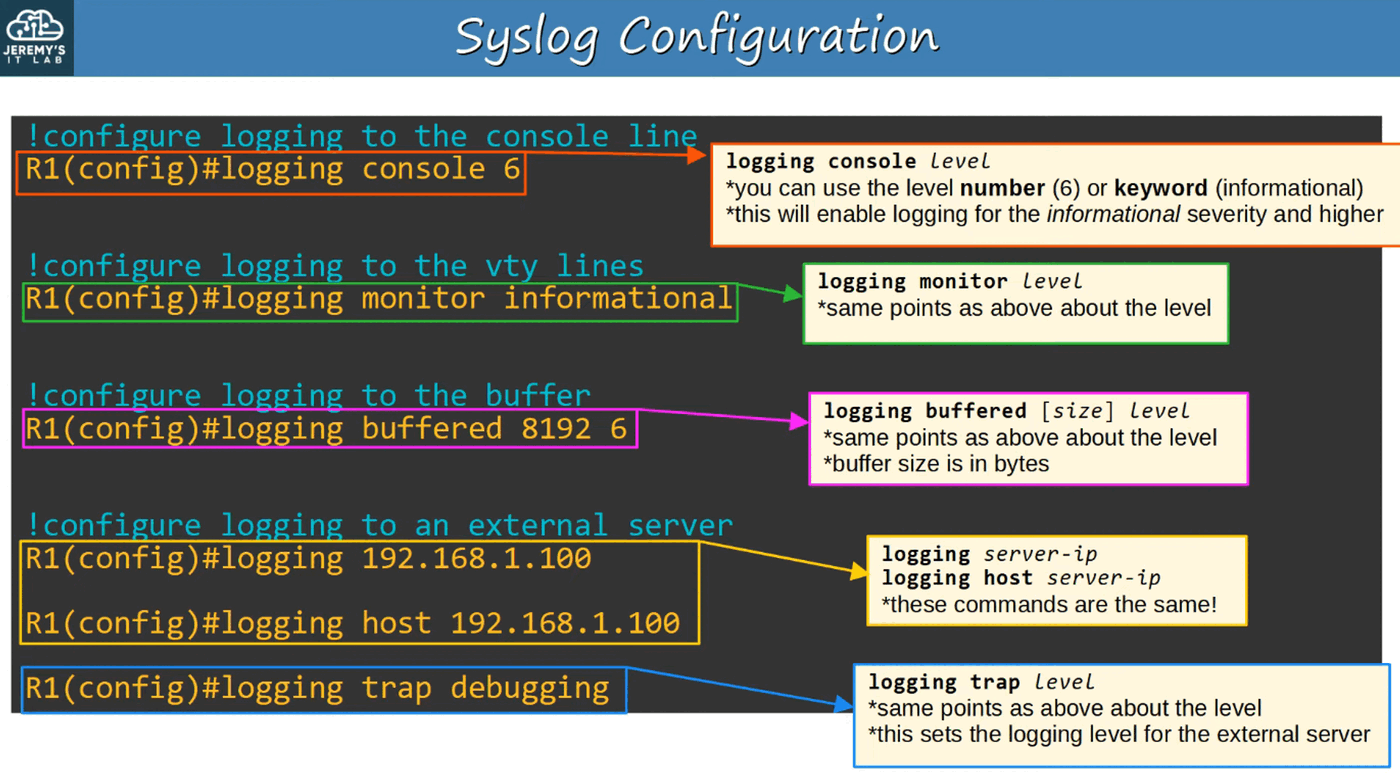
\includegraphics[keepaspectratio,alt={image}]{images/42-syslog/img-004.png}}
\end{figure}

\passthrough{\lstinline!level!} works from the chosen level and upward
toward Level 0 (EMERGENCY)

\passthrough{\lstinline!level!} or \passthrough{\lstinline!keyword!}
from the Severity Table works when choosing a level

\section{Terminal Monitor}\label{terminal-monitor}

\begin{itemize}
\tightlist
\item
  Even if \passthrough{\lstinline!logging monitor level!} is enabled, by
  default SYSLOG messages will not be displayed when connected via
  Telnet or SSH
\item
  For the messages to be displayed, you must use the following command:

  \begin{itemize}
  \tightlist
  \item
    \passthrough{\lstinline!R1\# terminal monitor!}
  \end{itemize}
\item
  The command must be used \textbf{every time you connect to the DEVICE
  via Telnet or SSH}
\end{itemize}

\section{Logging Synchronous}\label{logging-synchronous}

\begin{itemize}
\tightlist
\item
  By default, logging messages displayed in the CLI while you are in the
  middle of typing a command will result in something like this:
\end{itemize}

\begin{figure}
\centering
\pandocbounded{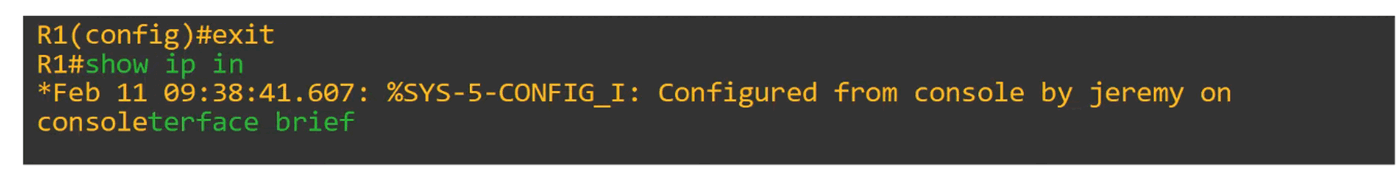
\includegraphics[keepaspectratio,alt={image}]{images/42-syslog/img-005.png}}
\end{figure}

\begin{itemize}
\tightlist
\item
  To prevent this, you should use
  \passthrough{\lstinline!logging synchronous!} on the appropriate
  \emph{line}
\end{itemize}

\begin{figure}
\centering
\pandocbounded{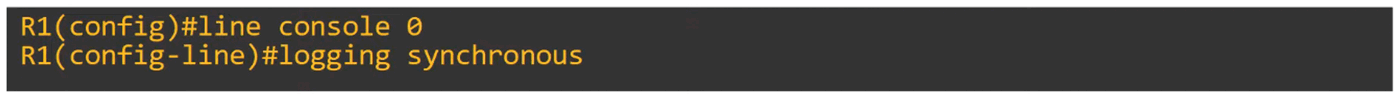
\includegraphics[keepaspectratio,alt={image}]{images/42-syslog/img-006.png}}
\end{figure}

\begin{itemize}
\tightlist
\item
  This will cause a new line to be printed if your typing is interrupted
  by a message
\end{itemize}

\begin{figure}
\centering
\pandocbounded{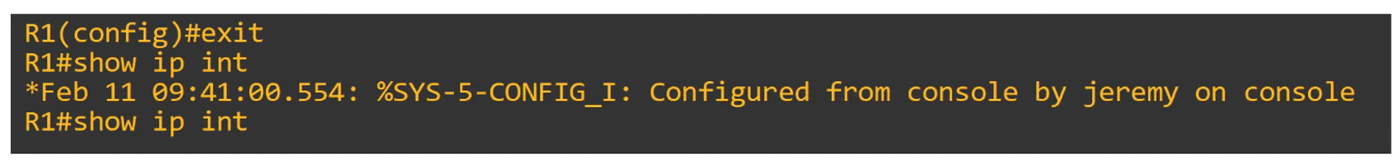
\includegraphics[keepaspectratio,alt={image}]{images/42-syslog/img-007.png}}
\end{figure}

SERVICE TIMESTAMPS and SERVICE SEQUENCE-NUMBERS

\begin{figure}
\centering
\pandocbounded{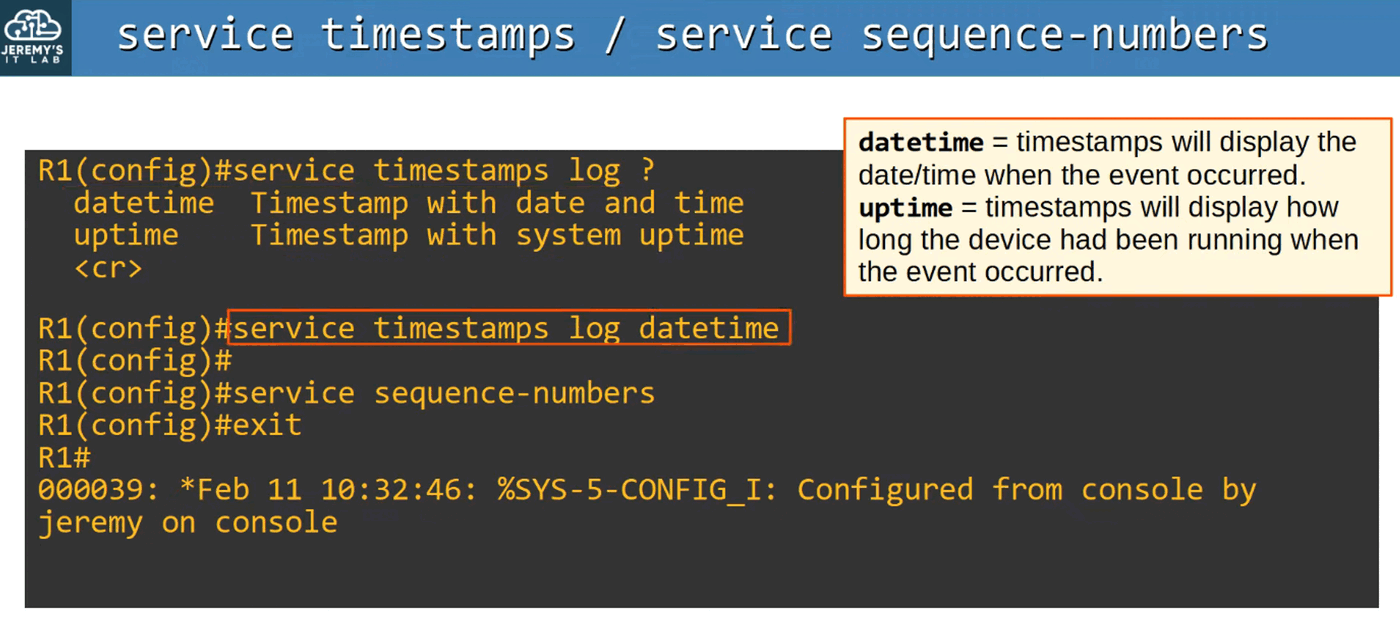
\includegraphics[keepaspectratio,alt={image}]{images/42-syslog/img-008.png}}
\end{figure}

SYSLOG versus SNMP

\begin{itemize}
\item
  SYSLOG and SNMP are both used for MONITORING and TROUBLESHOOTING of
  DEVICES. They are COMPLIMENTARY, but their FUNCTIONALITIES are
  different.
\item
  SYSLOG

  \begin{itemize}
  \tightlist
  \item
    Used for MESSAGE LOGGING
  \item
    Events that occur within the system are categorized based on
    FACILITY / SEVERITY and LOGGED
  \item
    Used for SYSTEM MANAGEMENT, ANALYSIS, and TROUBLESHOOTING
  \item
    Messages are sent from the DEVICES to the SERVER.

    \begin{itemize}
    \tightlist
    \item
      The SERVER can't actively pull information from the DEVICES (like
      SNMP `get') or modify variables (like SNMP `set')
    \end{itemize}
  \end{itemize}
\item
  SNMP

  \begin{itemize}
  \tightlist
  \item
    Used to retrieve and organize information about the SNMP managed
    DEVICES

    \begin{itemize}
    \tightlist
    \item
      IP ADDRESSES
    \item
      Current INTERFACE status
    \item
      Temperature
    \item
      CPU Usage
    \item
      etc\ldots{}
    \end{itemize}
  \item
    SNMP SERVERS can use \passthrough{\lstinline!Get!} to query the
    CLIENTS and \passthrough{\lstinline!Set!} to MODIFY variables on the
    CLIENTS
  \end{itemize}
\end{itemize}
